\documentclass{article}

\usepackage{fancyhdr} % Required for custom headers
\usepackage{lastpage} % Required to determine the last page for the footer
\usepackage{extramarks} % Required for headers and footers
\usepackage{graphicx} % Required to insert images
\usepackage{lipsum} % Used for inserting dummy 'Lorem ipsum' text into the template
\usepackage{ctable}

% Margins
\topmargin=-0.45in
\evensidemargin=0in
\oddsidemargin=0in
\textwidth=6.5in
\textheight=9.0in
\headsep=0.25in 

\linespread{1.1} % Line spacing

% Set up the header and footer
\pagestyle{fancy}
\chead{\hmwkTitle} % Top center header
\renewcommand\headrulewidth{0.4pt} % Size of the header rule
\renewcommand\footrulewidth{0.4pt} % Size of the footer rule

\setlength\parindent{0pt} % Removes all indentation from paragraphs

% Header and footer for when a page split occurs within a problem environment
\newcommand{\enterProblemHeader}[1]{
\nobreak\extramarks{#1}{#1 continued on next page\ldots}\nobreak
\nobreak\extramarks{#1 (continued)}{#1 continued on next page\ldots}\nobreak
}

% Header and footer for when a page split occurs between problem environments
\newcommand{\exitProblemHeader}[1]{
\nobreak\extramarks{#1 (continued)}{#1 continued on next page\ldots}\nobreak
\nobreak\extramarks{#1}{}\nobreak
}

\setcounter{secnumdepth}{0} % Removes default section numbers
\newcounter{homeworkProblemCounter} % Creates a counter to keep track of the number of problems

\newcommand{\homeworkProblemName}{}
\newenvironment{homeworkProblem}[1][Question \arabic{homeworkProblemCounter}]{ % Makes a new environment called homeworkProblem which takes 1 argument (custom name) but the default is "Problem #"
\stepcounter{homeworkProblemCounter} % Increase counter for number of problems
\renewcommand{\homeworkProblemName}{#1} % Assign \homeworkProblemName the name of the problem
\section{\homeworkProblemName} % Make a section in the document with the custom problem count
\enterProblemHeader{\homeworkProblemName} % Header and footer within the environment
}{
\exitProblemHeader{\homeworkProblemName} % Header and footer after the environment
}

\newcommand{\problemAnswer}[1]{ % Defines the problem answer command with the content as the only argument
\noindent\framebox[\columnwidth][c]{\begin{minipage}{0.98\columnwidth}#1\end{minipage}} % Makes the box around the problem answer and puts the content inside
}

\newcommand{\homeworkSectionName}{}
\newenvironment{homeworkSection}[1]{ % New environment for sections within homework problems, takes 1 argument - the name of the section
\renewcommand{\homeworkSectionName}{#1} % Assign \homeworkSectionName to the name of the section from the environment argument
\subsection{\homeworkSectionName} % Make a subsection with the custom name of the subsection
\enterProblemHeader{\homeworkProblemName\ [\homeworkSectionName]} % Header and footer within the environment
}{
\enterProblemHeader{\homeworkProblemName} % Header and footer after the environment
}
   
%----------------------------------------------------------------------------------------
%       NAME AND CLASS SECTION
%----------------------------------------------------------------------------------------

\newcommand{\hmwkTitle}{Assignment\ 1\ report} % Assignment title
\newcommand{\hmwkDueDate}{Friday,\ September\ 26,\ 2014} % Due date
\newcommand{\hmwkClass}{CS\ 5011}
\newcommand{\hmwkAuthorName}{Sure Manoj Kumar} % Your name

%----------------------------------------------------------------------------------------
%       TITLE PAGE
%----------------------------------------------------------------------------------------

\title{
\textmd{\textbf{\hmwkClass:\ \hmwkTitle}}\\
\normalsize\vspace{0.1in}\small{Due\ on\ \hmwkDueDate}\\
}

\author{\textbf{\hmwkAuthorName}}
\date{CS12B028} % Insert date here if you want it to appear below your name

%----------------------------------------------------------------------------------------

\begin{document}

\maketitle

\begin{homeworkProblem}[Question \arabic{homeworkProblemCounter}.]
Mean for class1 = [0]*10 \\
Mean for class2 = [3]*10 \\
Covariance matrix is same for both classes and the matrix is generated by taking each element as a random number between 0 and 3.and it is verified whether it is spherical or not.\\
Test data is chosen randomly from each class (400 data points from each class) and the remaining data is treated as the training data.\\
\end{homeworkProblem}


\begin{homeworkProblem}[Question \arabic{homeworkProblemCounter}.]
Based on the data set created in question 1(DS1),\\
Coefficients learnt = 0.19050926 , 0.00771853 , 0.07373751 , 0.0613499 ,  0.00560171 ,-0.00628388, 0.00203516 , 0.00403266 , 0.02744673 , 0.02573123 , 0.00418536 \\
Accuracy - 0.90375 \\
Precision - 0.906801007557\\
Recall - 0.9 \\
F-measure - 0.90338770389 \\

\end{homeworkProblem}

\begin{homeworkProblem}[Question \arabic{homeworkProblemCounter}.]
For the DS1, for k=5 the Accuracy is slightly higher compared to other values of k and the it's accuracy is slightly lower than that of regression on indicator variable.i.e; knn is doing worse than regression in this case.\\
for k=1\\
Accuracy - 0.84375\\
Precision - 0.846347607053\\
Recall - 0.84\\
F-measure -0.843161856964\\
for k=2\\
Accuracy - 0.82875\\
Precision - 0.894894894895\\
Recall - 0.745\\
F-measure -0.81309686221\\
for k=3\\
Accuracy - 0.87125\\
Precision - 0.872180451128\\
Recall - 0.87\\
F-measure -0.871088861076\\
for k=4\\
Accuracy - 0.8725\\
Precision - 0.909340659341\\
Recall - 0.8275\\
F-measure -0.866492146597\\
for k=5\\
Accuracy - 0.88625\\
Precision - 0.881481481481\\
Recall - 0.8925\\
F-measure -0.886956521739\\
for k=6\\
Accuracy - 0.88\\
Precision - 0.906417112299\\
Recall - 0.8475\\
F-measure -0.875968992248\\
for k=7\\
Accuracy - 0.885\\
Precision - 0.881188118812\\
Recall - 0.89\\
F-measure -0.885572139303\\
for k=8\\
Accuracy - 0.88375\\
Precision - 0.902887139108\\
Recall - 0.86\\
F-measure -0.880921895006\\
for k=9\\
Accuracy - 0.87875\\
Precision - 0.870415647922\\
Recall - 0.89\\
F-measure -0.880098887515\\
for k=10\\
Accuracy - 0.87625\\
Precision - 0.884910485934\\
Recall - 0.865\\
F-measure -0.874841972187\\

Best Fit for k=5:\\
Accuracy - 0.88625\\
Precision - 0.881481481481\\
Recall - 0.8925\\
F-measure -0.886956521739\\
\end{homeworkProblem}


\begin{homeworkProblem}[Question \arabic{homeworkProblemCounter}.]
In this problem, I have taken 2 mean vectors for two classes and 3 covaiance matrices (generated randomly)
The points are chosen  from each covariance matrix for each class based on given probabilities.\\
Mean1=[0]*10\\
Mean2=[3]*10\\
We can not say that which performs better because it largely depends on what the actual data set is rather than how you generate it, but for mixture of guassians knn works better than linear classifier if we take different means for different covariance matrices,beacause there is a high chance that we can not find a line to seperate those classes.But in the case I have chosen,linear  classifier works slightly better because there are only two means but different covariance matrices.\\

{\bf performance Results:}\\

{\bf Using linear classifier:}\\
Coefficients learnt:
 0.18627366  0.02848674  0.02265773  0.02526162  0.02790363  0.00238386
  0.03325447  0.02182644  0.01192047  0.01345345  0.01415136\\
Accuracy - 0.885\\
Precision - 0.892857142857 \\
Recall - 0.875\\
F-measure - 0.883838383838\\

{ \bf Using knn:}\\
Accuracy - 0.86625\\
Precision - 0.865336658354\\
Recall - 0.8675\\
F-Measure - 0.866416978777\\

\end{homeworkProblem}

\begin{homeworkProblem}[Question \arabic{homeworkProblemCounter}.]
In this question, we are asked to fill the missing values with mean.But mean is not a really good choice ,if the data is completely skewed(such as one noisy point which has a really large value can increase the mean of the entire data set considerably.Instead , we can use median to fill the data set so that those noisy points will not have much effect.
But the given data set is not so noisy, so I have used the mean to fill the missing attributes.
\end{homeworkProblem}

\begin{homeworkProblem}[Question \arabic{homeworkProblemCounter}.]
5 80-20 different splits are done by choosing random 20 percent from the dataset and set that as testdata and the remaining as training data and the process is repeated 5 times.\\

Average mse - 0.01848167098 ;  Average RSS - 7.37\\
mse1 - 0.018474853191; rss1 - 7.37\\
mse2 - 0.0204983378639; rss2 - 8.17\\
mse3 - 0.0209688850415; rss3 - 8.36\\
mse4 - 0.0155163266286; rss4 - 6.19\\
mse5 - 0.0169499521748; rss5 - 6.76\\
\end{homeworkProblem}

\begin{homeworkProblem}[Question \arabic{homeworkProblemCounter}.]
The below values are for lambda = 2 (which is observed to have less  mean rss compared to others)\\
average mse - 0.0176589717892;Average RSS - 7.04 \\
mse1 - 0.0183201292463;  rss1 - 7.30\\
mse2 - 0.01876789375;  rss2 - 7.48\\
mse3 - 0.0192973920872;  rss3 - 7.69\\
mse4 - 0.0148353674319;  rss4 - 5.91\\
mse5 - 0.0170740764304;  rss5 - 6.81\\
\end{homeworkProblem}

\begin{homeworkProblem}[Question \arabic{homeworkProblemCounter}.]
Precision for class0 - 0.611940298507\\
Precision for class1 - 0.613065326633\\
Recall for class0- 0.615\\
Recall for class1- 0.61\\
F-measure for class0 - 0.6134\\
f-measure for class1 - 0.6115\\
Figure1 is the dataset projection in 3d.\\
Figure2 has both points in the derived feature space and also the classifier.\\
The classifier is actually a point(in Figure 2), but the point was not visible when plotted. So ,I have used a line that passes through the classifier point for the representation.
\end{homeworkProblem}

\begin{homeworkProblem}[Question \arabic{homeworkProblemCounter}.]
Precision for class0- 1.0\\
Precision for class1- 1.0\\
Recall for class 0- 1.0\\
Recall for class 1- 1.0\\
F-measure for class 0- 1.0\\
F-meaure for class 1 - 1.0\\
Figure1 is the dataset projection in 3d.\\
Figure3 represents the extracted feature set along with the classifier(red point)\\
Based on the above two feature extraction methods,it can be clearly seen that lda is performing much better compared to pca.This is mainly because of the given data set,From the plot of the given data set, the points are roughly present on two parallel lines with some guassian noise,also they are present within the same range ,so when we perform pca and apply linear regression, both the classes merge and classifying will not be accurate.Whereas in lda,the data sets are linearly seperable so we get 100percent accurate measurements.
\end{homeworkProblem}
\begin{figure}[h!]
\centering
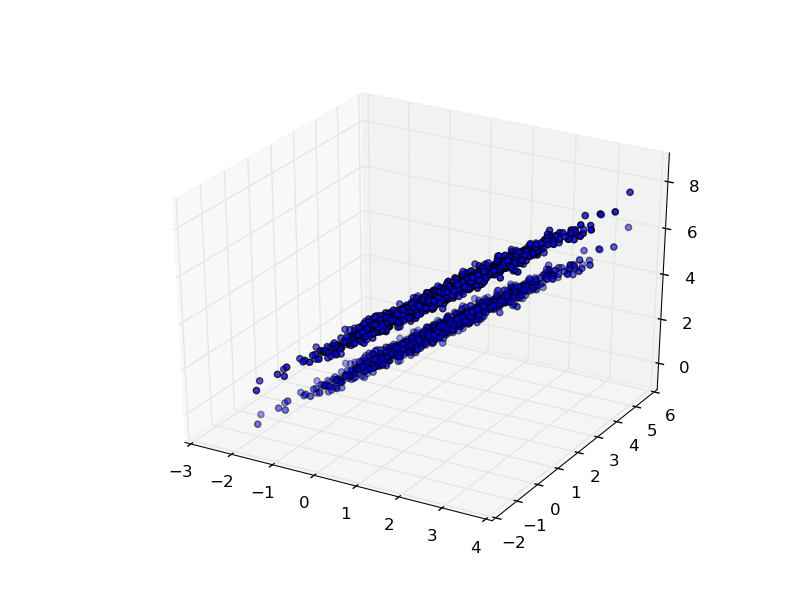
\includegraphics[width=0.5\textwidth]{figure_1.png}
\caption{Data Set}
\end{figure}
\begin{figure}[h!]
\centering
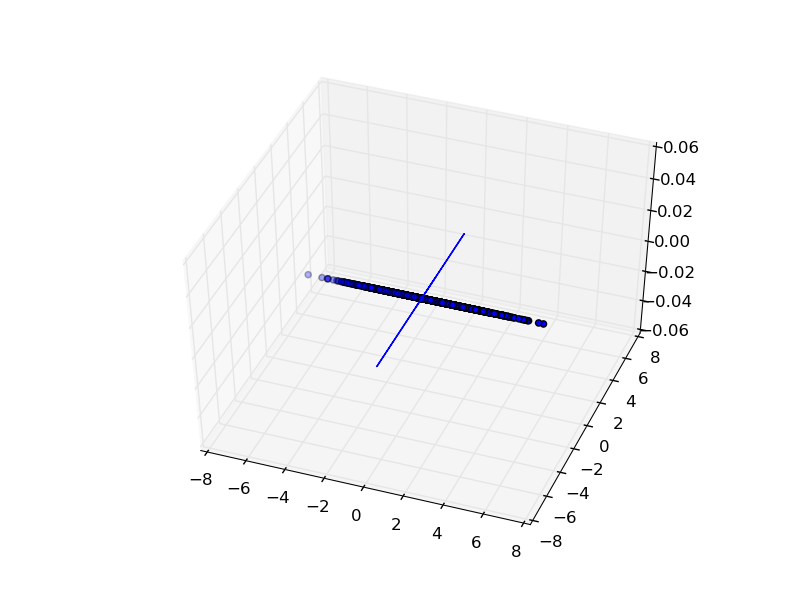
\includegraphics[width=0.5\textwidth]{figure_2.png}
\caption{Data Set in the derived feature space(pca)}
\end{figure}
\begin{figure}[h!]
\centering
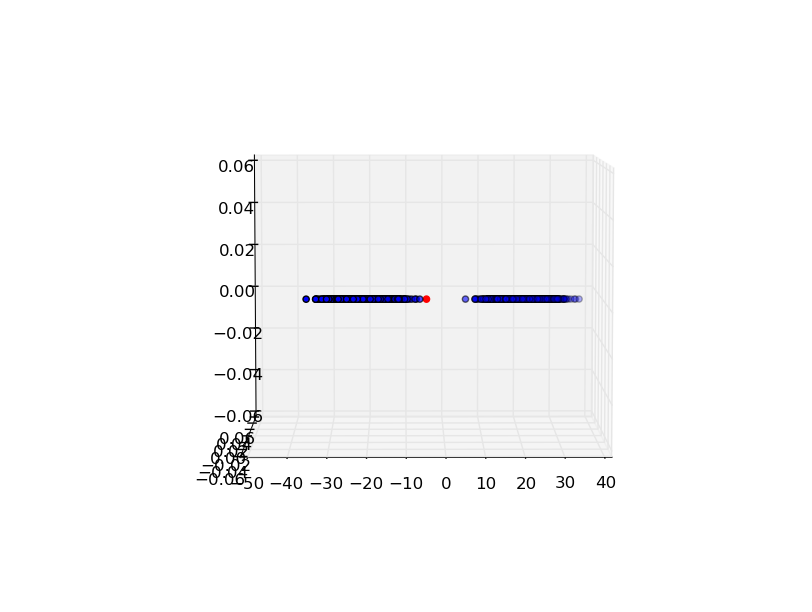
\includegraphics[width=0.5\textwidth]{figure_3.png}
\caption{Data Set in the derived feature space(lda)}
\end{figure}
\end{document}